
\chapter{Markov Decision Process}

% https://trunghng.github.io/artificial-intelligent/reinforcement-learning/2021/06/27/mdp-bellman-eqn.html


\subsection{What is Reinforcement Learning?}

Say, there is an unknown environment that we're trying to put an agent on. By 
interacting with the agent through taking actions that gives rise to rewards 
continually, the agent learns a policy that maximize the cumulative rewards.

Reinforcement Learning (RL), roughly speaking, is an area of Machine Learning 
that describes methods aimed to learn a good strategy (called policy) for the 
agent from experimental trials and relative simple feedback received. With the 
optimal policy, the agent is capable to actively adapt to the environment to
maximize future rewards.

\subsection{Return}

The goal of agent is to maximize the cumulative reward in the long run. In 
general, we seek to maximize the expected return.

\begin{definition} {\rm\bf (Return)}
The return $G_t$ is the total discounted reward from $t$
\begin{equation}
G_t=R_{t+1}+\gamma R_{t+2}+\gamma^2 R_{t+3}+\dots=\sum_{k=0}^{\infty}\gamma^k R_{t+k+1},
\end{equation}
where $\gamma\in[0,1]$ is called discount rate (or discount factor).
\end{definition}

The discount rate $\gamma$ determines the present value of future rewards: a 
reward received $k$ time steps in the future is worth only $\gamma^{k-1}$ times 
what it would be worth if it were received immediately. And also, it provides 
mathematical convenience since as $k\rightarrow\infty$ then $\gamma^k\rightarrow 0$.


\subsection{Policy}

Policy, which is denoted as $\pi$, is the behaviour function of the agent. $\pi$ 
is a mapping from states to probabilities of selecting each possible action. In 
other words, it lets us know which action to take in the current state $s$ and can 
be either deterministic or stochastic.

\begin{itemize}
%\setlength{\itemsep}{0pt}
%\setlength{\parsep}{0pt}
\setlength{\parskip}{0pt}
\item[-]
Deterministic policy:
$\quad\pi(s)=a$

\item[-]
Stochastic policy: 
$\quad\pi(a|s)=P(A_t=a|S_t=s)$

\end{itemize}


\subsection{Value Function}

Value function measures how good a particular state is (or how good it is to 
perform a given action in a given state).

\begin{definition} {\rm\bf (state-value function)}
The state-value function of a state $s$ under a policy $\pi$, denoted as $v_\pi(s)$, 
is the expected return starting from state $s$ and following $\pi$ thereafter:
\begin{equation}
v_\pi(s)=\mathbb{E}_\pi[G_t|S_t=s]
\end{equation}
\end{definition}

\begin{definition} {\rm\bf (action-value function)}
Similarly, we define the value of taking action a in state $s$ under a policy $\pi$, 
denoted as $q_\pi(s,a)$, as the expected return starting from $s$, taking the 
action $a$, and thereafter following policy $\pi$:
\begin{equation}
q_\pi(s,a)=\mathbb{E}_\pi[G_t|S_t=s,A_t=a]
\end{equation}
Since we follow the policy $\pi$, we have that
\begin{equation}
v_\pi(s)=\sum_{a\in\mathcal{A}}q_\pi(s,a)\pi(a|s)
\end{equation}
\end{definition}



\section{Markov Decision Processes}

{\bf Markov decision processes (MDPs)} formally describe an environment for RL. 
And almost all RL problems can be formalised as MDPs.

\begin{definition} {\rm\bf (MDP)}
A Markov Decision Process is a tuple $<\mathcal{S}, \mathcal{A}, \mathcal{P}, 
\mathcal{R}, \gamma>$
\begin{itemize}
%\setlength{\itemsep}{0pt}
%\setlength{\parsep}{0pt}
\setlength{\parskip}{0pt}
\item[-]
$\mathcal{S}$ is a set of states called state space

\item[-]
$\mathcal{A}$ is a set of actions called action space

\item[-]
$\mathcal{P}$ is a state transition probability matrix \\
$\mathcal{P}^a_{ss'}=P(S_{t+1}=s'|S_t=s,A_t=a)$

\item[-]
$\mathcal{R}$ is a reward function \\
$ \mathcal{R}^a_s=\mathbb{E}\left[R_{t+1}|S_t=s,A_t=a\right]$

\item[-]
$\gamma\in[0, 1]$ is a discount factor for future reward
\end{itemize}
\end{definition}


\subsection{Optimal Policy and Optimal Value Function}

For finite MDPs (finite state and action space), we can precisely define an 
optimal policy. Value functions define a partial ordering over policies. A 
policy $\pi$ is defined to be better than or equal to a policy $\pi'$ if its 
expected return is greater than or equal to that of $\pi'$ for all states. In 
other words, 
\begin{equation} 
\pi\geq\pi'\iff v_\pi(s)\geq v_{\pi'} \forall s\in\mathcal{S} 
\end{equation}

\begin{theorem} {\rm\bf (Optimal policy)}
For any MDP, there exists an optimal policy $\pi_*$ that is better than or equal 
to all other policies, 
\begin{equation} 
\pi_*\geq\pi,\forall\pi 
\end{equation}
\end{theorem}

The proof of the above theorem is gonna be provided in another section since we 
need some additional tools to do that.

There may be more than one optimal policy, they share the same state-value function, 
called optimal state-value function though. 
\begin{equation} 
v_*(s)=\max_{\pi}v_\pi(s) 
\end{equation} 
Optimal policies also share the same action-value function, call optimal action-value 
function 
\begin{equation} 
q_*(s,a)=\max_{\pi}q_\pi(s,a) 
\end{equation}


\subsection{Bellman Equations}

A fundamental property of value functions used throughout RL is that they satisfy 
recursive relationships 
\begin{align*} 
v_\pi(s)&\doteq \mathbb{E}_\pi[G_t|S_t=s] \\
&=\mathbb{E}_\pi[R_t+\gamma G_{t+1}|S_t=s] \\
&=\sum_{s',r,g',a}p(s',r,g',a|s)(r+\gamma g') \\
&=\sum_{a}p(a|s)\sum_{s',r,g'}p(s',r,g'|a,s)(r+\gamma g') \\
&=\sum_{a}\pi(a|s)\sum_{s',r,g'}p(s',r|a,s)p(g'|s',r,a,s)(r+\gamma g') \\
&=\sum_{a}\pi(a|s)\sum_{s',r}p(s',r|a,s)\sum_{g'}p(g'|s')(r+\gamma g') \\
&=\sum_{a}\pi(a|s)\sum_{s',r}p(s',r|a,s)\left[r+\gamma\sum_{g'}p(g'|s')g'\right] \\
&=\sum_{a}\pi(a|s)\sum_{s',r}p(s',r|a,s)\left[r+\gamma v_\pi(s')\right], 
\end{align} 
where $p(s',r|s,a)=P(S_{t+1}=s',R_{t+1}=r|S_t=s,A_t=a)$, which defines the dynamics 
of the MDP. The last equation is called the Bellman equation for $v_\pi(s)$. It 
expresses a relationship between the value state $s$, $v_\pi(s)$ and the values of 
its successor states $s'$, $v_\pi(s')$.

Similarly, we define the Bellman equation for $q_\pi(s,a)$ 
\begin{align*} 
q_\pi(s,a)&\doteq\mathbb{E}_\pi[G_t|S_t=s,A_t=a] \\
&=\mathbb{E}_\pi[R_t+\gamma G_{t+1}|S_t=s,A_t=a] \\
&=\sum_{s',r}p(s',r|s,a)\left[r+\gamma\sum_{a'}\pi(a'|s')q_\pi(s',a')\right] 
\end{align}


\subsection{Bellman Backup Diagram}

Backup diagram of state-value function and action-value function respectively


\begin{tikzpicture}[->,>=stealth',level/.style={sibling distance = 5cm/#1,
  level distance = 1.5cm}] 
\node [arn_r] {}
    child{ node [arn_n] (test0) {}
        {
            child{ node [arn_r] {}
                {
                edge from parent node[above left] {$r$}
                edge from parent node[below left] (A) { \makebox[6em][l]{$v_\pi(s') \leftarrowtail s'$} }
                }
            }
            child{ node [arn_r] {} }
            edge from parent node[below left] (A) { \makebox[4em][l]{$a$} }
        }% edge from parent node[left] {$r$} %for a named pointer
    }
    child{ node [arn_n] (test1) {}
            child{ node [arn_r] {} }
            child{ node [arn_r] {} }
	}edge from parent node[left] (A) {\makebox[5em][l]{$v_\pi(s) \leftarrowtail s$}}
    
    ;

    %\filldraw[red] (A) circle[radius=1pt];
\end{tikzpicture}



\begin{tikzpicture}[->,>=stealth',level/.style={sibling distance = 5cm/#1,
  level distance = 1.5cm}] 
\node [arn_n] {}
    child{ node [arn_r] (test0) {}
        {
            child{ node [arn_n] {}
                {
                % edge from parent node[above left] {$r$}
                edge from parent node[below left] (A) { \makebox[8em][l]{$q_\pi(s',a') \leftarrowtail a'$} }
                }
            }
            child{ node [arn_n] {} }
            edge from parent node[below left] (A) { \makebox[4em][l]{$s'$} }
        } edge from parent node[left] {$r$} %for a named pointer
    }
    child{ node [arn_r] (test1) {}
            child{ node [arn_n] {} }
            child{ node [arn_n] {} }
	}edge from parent node[left] (A) {\makebox[7em][l]{$q_\pi(s,a) \leftarrowtail s, a$}}
    
    ;

    %\filldraw[red] (A) circle[radius=1pt];
\end{tikzpicture}


\subsection{Bellman Optimality Equations}

The optimal policy can be found once we have found the optimal state-value function 
$v_*$ and the optimal action-value function $q_*$.
Since $v_*$ is the value function for a policy, it must satisfy the Bellman equation 
for {\bf state-values}. Moreover, it is also the optimal value function, then we have 
\begin{align} 
v_*(s)&=\max_{a\in\mathcal{A}(s)}q_{\pi_*}(s,a)  \notag \\
&=\max_{a}\mathbb{E}_{\pi_*}[G_t|S_t=s,A_t=a]  \notag \\
&=\max_{a}\mathbb{E}_{\pi_*}[R_{t+1}+\gamma G_{t+1}|S_t=s,A_t=a]  \notag \\
&=\max_{a}\mathbb{E}[R_{t+1}+\gamma v_*(S_{t+1})|S_t=s,A_t=a]  \label{mdp_bellman_optimality_equation_1} \\
&=\max_{a}\sum_{s',r}p(s',r|s,a)[r+\gamma v_*(s')]  \label{mdp_bellman_optimality_equation_2}  
\end{align} 
The last two equations are two forms of the Bellman optimality equation for $v_*$. 
Similarly, we have the Bellman optimality equation for {\bf action-value} $q_*$ 
\begin{align} 
q_*(s,a)&=\mathbb{E}\left[R_{t+1}+\gamma\max_{a'}q_*(S_{t+1},a')|S_t=s,A_t=a\right] \\
&=\sum_{s',r}p(s',r|s,a)\left[r+\gamma\max_{a'}q_*(s',a')\right] 
\end{align}


\subsection{Bellman Optimality Equation vs Optimal Policy}
% https://yangyangfu.github.io/learning/reinforcement%20learning/2020/05/09/Bellman-Equation/

The ultimate goal of RL is to find the optimal policy. But how does the Bellman 
optimality equation relate to the optimal policy?

Once we find out the optimal state-value $v_*$, it is relatively easy to determine 
an optimal policy. For each state $s$, there will be one or more actions at which 
the maximum is obtained from the Bellman optimality equation. Any policy that assigns 
nonzero probability only to these actions is an optimal policy. You can think of this 
as a one-step search. If we have the optimal state-value function $v_*$, then the 
actions that appear best after a one-step search will be optimal actions.

Let's now retreat all these in another way: any policy that is greedy with respect to 
the optimal evaluation function $v_*$ is an optimal policy. The term greedy is used 
in computer science to describe any search or decision procedure that selects 
alternatives based only on local or immediate considerations, without considering the 
possibility that such a selection may prevent future access to even better alternatives. 
Consequently, it describes policies that select actions based only on their short-term 
consequences. The beauty of $v_*$ is that if one uses it to evaluate the short-term 
consequences of actions��specifically, the one-step consequences��then a greedy policy is 
actually optimal in the long-term sense in which we are interested because $v_*$ already 
takes into consideration the reward consequences of all possible future behavior. By 
means of $v_*$, the optimal expected long-term return is turned into a quantity that is 
locally and immediately available for each state. Hence, a one-step-ahead search yields 
the long-term optimal actions.

Having $q_*$ makes choosing optimal actions even easier. With $q_*$, the agent does not 
even have to do a one-step-ahead search: for any state $s$, it can simply find any 
action that maximizes $q_*(s, a)$. The action-value function actively caches the results 
of all one-step-ahead searches. It provides the optimal expected long-term return as a 
value that is locally and immediately available for each state�Caction pair. Hence at the 
cost of representing a function of state�Caction pairs, instead of just of states, the 
optimal actionvalue function allows optimal actions to be selected without having to 
know anything about possible successor states and their values, that is, without having 
to know anything about the environment's dynamics.



\subsection{Backup diagram for $v_*$ and $q_*$}


\begin{figure}[!htb]
\centering
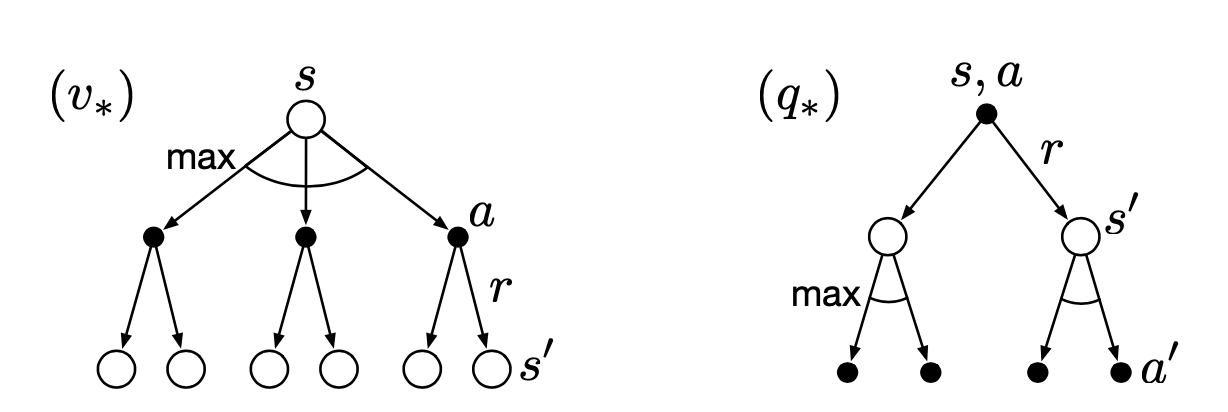
\includegraphics[scale=0.618]{pix/opt.png}
\caption{backup diagram for $v_*$ and $q_*$}
%\label{fig:label}
\end{figure}


\subsection{References}

\cite{silver2015}

% https://lilianweng.github.io/lil-log/2018/02/19/a-long-peek-into-reinforcement-learning.html

% https://deepmind.com/research/case-studies/alphago-the-story-so-far

